\chapter{Introduction}
\lecture{1}{13/1}

We have already studied networks, 
which shows us \emph{how} to communicate with different devices.
The focus of distributed systems is more on how we connect networked components
that are geographically dispersed to form a powerful, high-performance, and
reliable system.

\begin{definition}[Distributed system]
    A \textbf{distributed system} is a collection of independent components,
    such as
    \begin{enumerate}
        \item hardware;
        \item software; and
        \item web services.
    \end{enumerate}
    These components work together to offer a single coherent system to users.
\end{definition}

\begin{figure}
    \centering
    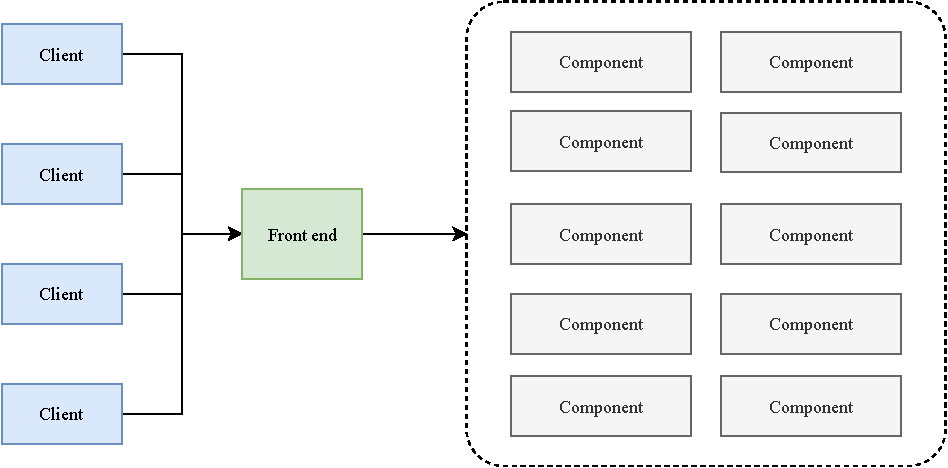
\includegraphics[width=0.8\linewidth]{images/simple-distributed-system.pdf}
    \caption{A simplified view of a distributed system.}
    \label{fig:simple-distributed-system}
\end{figure}

\begin{example}
    Figure \ref{fig:simple-distributed-system} illustrates a simple distributed system. 
    The components in a distributed systen may \emph{not} be the same,
    this makes interactions between the more complicated.
    The figure depicts a \textbf{front-end} between the users and the components;
    the front-end provides an interface to access the system as a whole instead of
    each individual component.
    We will introduce models of distributed systems in due time.
\end{example}

\paragraph{Benefits of distributed systems}
\begin{enumerate}
    \item Rapid system development by
        reusing existing components 
        (instead of buying new ones).

    \item Construct low-cost, 
        scalable systems by linking lots of low-cost machines.

    \item Improve system reliability 
        and availability by having redundant components.
\end{enumerate}
